% !TEX root = ../Dokumentation.tex
\subsection{Antrieb}

\textbf{Funktionsbeschrieb}\\[0.2cm]
Als Antrieb wird ein DC-Getriebemotor verwendet, der an der Unterseite montiert wird und für die Vor- sowie Rückwärtbewegungen des Fahrzeugs zuständig ist.
Die aktuelle Drehzahl des Motors wird von einem Encoder erfasst. Dieser wiederum sendet die gemessenen Daten an den Microcontroller der schlussendlich die Anzahl Umdrehungen reguliert.\\[0.2cm]
\textbf{Komponentenbeschrieb}
\begin{figure}[H]
\centering
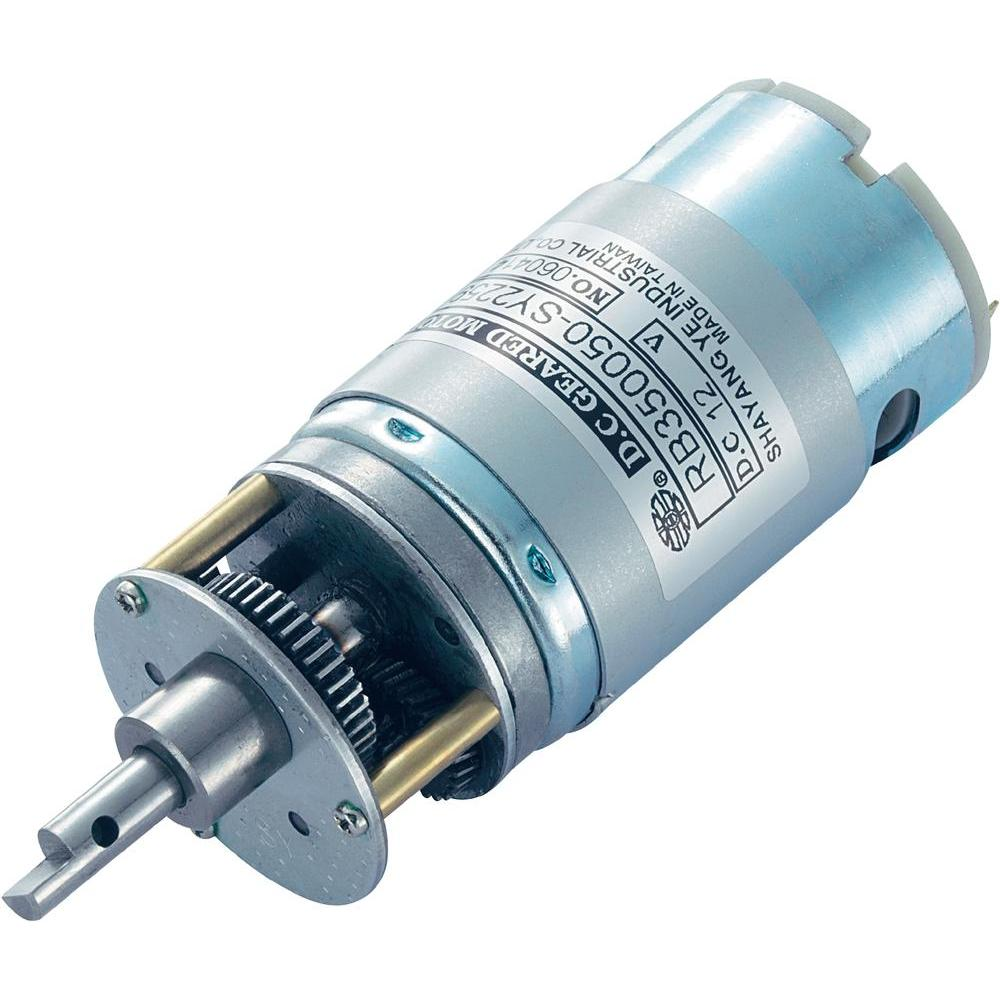
\includegraphics[width=0.5\textwidth]{03_Loesungskonzept/pictures/antrieb.jpg}
\caption{Antrieb  (Quelle:http://www.conrad.ch)}	
\end{figure}\flushleft
Als voraussichtlicher Favorit, wurde ein Hochleistungsgetriebemotor von Modelcraft ausgewählt. Die technischen Daten sind folgende:
\begin{itemize}
\item Leerlaufstrom: 0.32 A
\item Last-Drehzahl: 317 U/min
\item Leerlauf-Drehzahl: 333 U/min
\item Betriebsspannung: 12 V DC
\item Spitzendrehmoment: 2.23 Nm
\item Max. Laststrom: 0.7 A
\end{itemize}
\textbf{Begründung}\\[0.2cm]
Der ausgewählte Motor punktet vor allem aufgrund seiner kleinen und kompakten Bauform. Da der Montageort für den Antrieb am Fahrzeug nicht verändert werden kann, ohne umständliche Wellen zu installieren, ist die Baugrösse relativ beschränkt.
Ein weiterer Punkt ist, dass er sich als Gleichstrommotor leicht ansteuern lässt und damit die Handhabung vereinfacht.
Zudem zeichnet er sich mit einer hohen Drehzahl und grossem Drehmoment aus und ist dennoch verhältnismässig günstig in der Anschaffung.
